\documentclass[10pt]{article}
\usepackage[utf8]{inputenc}
\usepackage[T1]{fontenc}
\usepackage{amsmath}
\usepackage{amsfonts}
\usepackage{amssymb}
\usepackage[version=4]{mhchem}
\usepackage{stmaryrd}
\usepackage{graphicx}
\usepackage[export]{adjustbox}
\graphicspath{ {./images/} }
\usepackage{caption}

\begin{document}
\captionsetup{singlelinecheck=false}
\section*{CHEMSITRY}
\section*{SECTION-A}
\begin{enumerate}
  \setcounter{enumi}{30}
  \item Which of the following compounds would give the following set of qualitative analysis ?\\
(i) Fehling's Test : Positive\\
(ii) Na fusion extract upon treatment with sodium nitroprusside gives a blood red colour but not\\
(1)\\

\includegraphics{smile-5fb7dece4a6928835dba589aa888a4e727ea31b3}\\
(2)\\

\includegraphics{smile-e51edaf5182eb11c95700c4a34f485beffafd59a}\\
(3)\\

\includegraphics{smile-3b46b3699aa611d491466424158c6cf3b29cb5ca}\\
(4)\\

\includegraphics{smile-cdac5ec57768bf7e7f3596a0c88a4ce3c9db3724}
\end{enumerate}

Official Ans. by NTA (4)\\
Allen Ans. (4)\\
Sol. Aromatic aldehydes do not give Fehling's test..\\
Both nitrogen and sulfur must be present to obtain blood red colour Sodium nitroprusside gives blood red colour with S \& N.\\
32. What is the correct order of acidity of the protons marked \(\mathrm{A}-\mathrm{D}\) in the given compounds?\\

\includegraphics{smile-7b1d473e469de3cfe09f09cfeb0397c15aff2a33}\\
(1) \(\mathrm{H}_{\mathrm{C}}>\mathrm{H}_{\mathrm{D}}>\mathrm{H}_{\mathrm{B}}>\mathrm{H}_{\mathrm{A}}\)\\
(2) \(\mathrm{H}_{\mathrm{C}}>\mathrm{H}_{\mathrm{D}}>\mathrm{H}_{\mathrm{A}}>\mathrm{H}_{\mathrm{B}}\)\\
(3) \(\mathrm{H}_{\mathrm{D}}>\mathrm{H}_{\mathrm{C}}>\mathrm{H}_{\mathrm{B}}>\mathrm{H}_{\mathrm{A}}\)\\
(4) \(\mathrm{H}_{\mathrm{C}}>\mathrm{H}_{\mathrm{A}}>\mathrm{H}_{\mathrm{D}}>\mathrm{H}_{\mathrm{B}}\)

Official Ans. by NTA (2)\\
Allen Ans. (2)\\
Sol. acidity of an acid depends upon the stability of its conjugate base

\section*{TEST PAPER WITH SOLUTION}

\includegraphics{smile-877b221b4ca676d5a4826074c13eb1926f2a56fe}\\

\includegraphics{smile-c3262ca962b5b700c1166c202fc140101f8da8d7}\\

\includegraphics{smile-28714c5c2c0f0b6a010585f7641a10e3b3ecf872}\\
\(>\)\\

\includegraphics{smile-51331149167c6d8b41c4b2a90e0ee33f9aaa67ca}\\
33. Given below are two statements : one is labelled as Assertion (A) and the other is labelled as Reason (R).

Assertion (A) : Ketoses give Seliwanoff's test faster than Aldoses.

Reason (R) : Ketoses undergo \(\beta\)-elimination followed by formation of furfural.

In the light of the above statements, choose the correct answer from the options given below :\\
(1) (A) is false but (R) is true\\
(2) Both (A) and (R) are true and (R) is the correct explanation of (A)\\
(3) (A) is true but (R) is false\\
(4) Both (A) and (R) are true but (R) is not the correct explanation of (A)

Official Ans. by NTA (3)\\
Allen Ans. (3)\\
Sol. Seliwanoff 's test is a differentiating test for Ketose and aldose. This test relies on the principle that the keto hexose are more rapidly dehydrated to form 5-hydroxy methyl furfural when heated in acidic medium which on condensation with resorcinol, Cherry red or brown red coloured complex is formed rapidly indicating a positive test.\\
34. In the extraction of copper, its sulphide ore is heated in a reverberatory furnace after mixing with silica to :\\
(1) separate CuO as \(\mathrm{CuSiO}_{3}\)\\
(2) remove calcium as \(\mathrm{CaSiO}_{3}\)\\
(3) decrease the temperature needed for roasting of \(\mathrm{Cu}_{2} \mathrm{~S}\)\\
(4) remove FeO as \(\mathrm{FeSiO}_{3}\)

Official Ans. by NTA (4)\\
Allen Ans. (4)\\
Sol. The copper ore contains iron, it is mixed with silica before heating in reverberatory furnace. FeO slags off as \(\mathrm{FeSiO}_{3}\).

\[
\mathrm{FeO}+\mathrm{SiO}_{2} \longrightarrow \mathrm{FeSiO}_{3}
\]

\begin{enumerate}
  \setcounter{enumi}{34}
  \item Amongst the following compounds, which one is an antacid ?\\
(1) Ranitidine\\
(2) Meprobamate\\
(3) Terfenadine\\
(4) Brompheniramine
\end{enumerate}

Official Ans. by NTA (1)\\
Allen Ans. (1)\\
Sol. 1. Ranitidine: Antacid\\
2. Meprobamate: Tranquilizer\\
3. Terfenadine: Antihistamine\\
4. Brompheniramine: Antihistamine\\
36. The major products 'A' and 'B', respectively, are\\
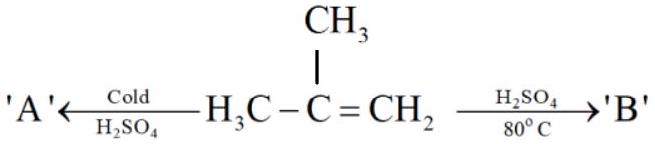
\includegraphics[max width=\textwidth, center]{2025_10_03_730bb016301631b89e24g-2(1)}

(1)\\

\includegraphics{smile-055841fec1150ab1805a6bea6a3d1c83b73169e6}\\

\includegraphics{smile-501abe300a30cce3411f2415b1e14a8ee1f2e5c0}

(2)\\

\includegraphics{smile-b323eee7c7e4f6f235afba88401d5cc9a0654b8b}\\
3\\

\includegraphics{smile-b9d10b9963ca666b0ef991d8ed0ba61a4b52f092}

(3)\\

\includegraphics{smile-b3741614ea9b80f0bd212e612d9716861cf65f3d}\\

\includegraphics{smile-a845eaaa876bc659c15f9fea21017c44dbc242f4}

(4)\\

\includegraphics{smile-09be8a2dcfe11a07947844dae03d766476d20cc7}\\
\&\\

\includegraphics{smile-287cf0eb178cdb8e0d9928608ff000c0aed60368}

\section*{Official Ans. by NTA (1)}
Allen Ans. (1)

Sol.\\
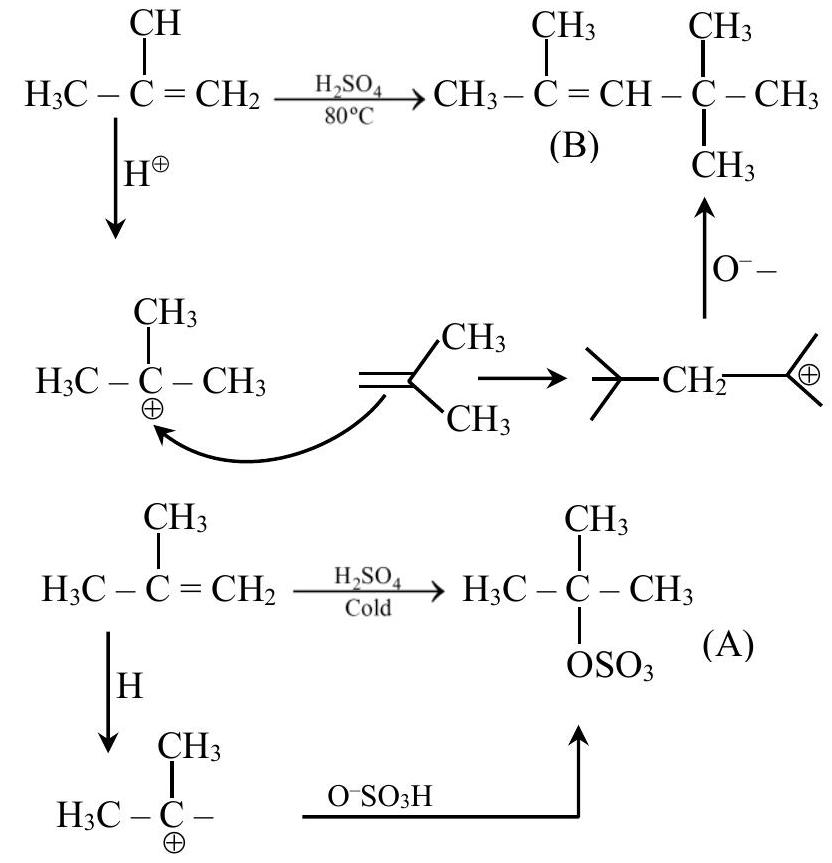
\includegraphics[max width=\textwidth, center]{2025_10_03_730bb016301631b89e24g-2(4)}\\
37. Benzyl isocyanide can be obtained by :\\
(A)\\
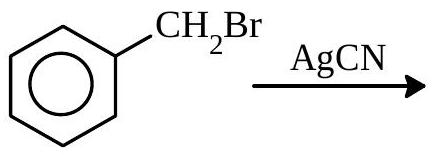
\includegraphics[max width=\textwidth, center]{2025_10_03_730bb016301631b89e24g-2(3)}\\
(B)\\
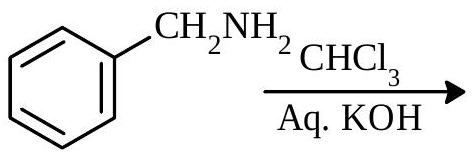
\includegraphics[max width=\textwidth, center]{2025_10_03_730bb016301631b89e24g-2}\\
(C)\\
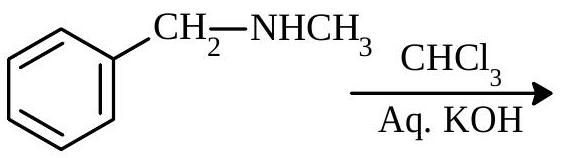
\includegraphics[max width=\textwidth, center]{2025_10_03_730bb016301631b89e24g-2(5)}\\
(D)\\
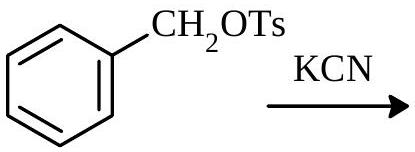
\includegraphics[max width=\textwidth, center]{2025_10_03_730bb016301631b89e24g-2(2)}

Choose the correct answer from the options given below :\\
(1) A and D\\
(2) Only B\\
(3) A and B\\
(4) B and C

Official Ans. by NTA (3)\\
Allen Ans. (3)

Sol.\\
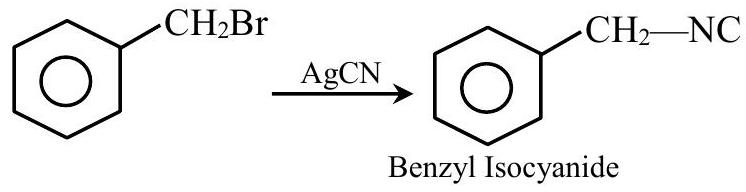
\includegraphics[max width=\textwidth, center]{2025_10_03_730bb016301631b89e24g-3(4)}\\
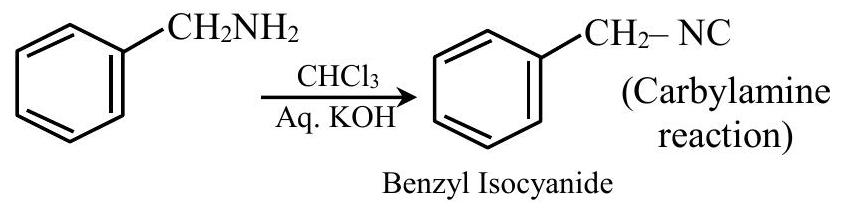
\includegraphics[max width=\textwidth, center]{2025_10_03_730bb016301631b89e24g-3(3)}\\
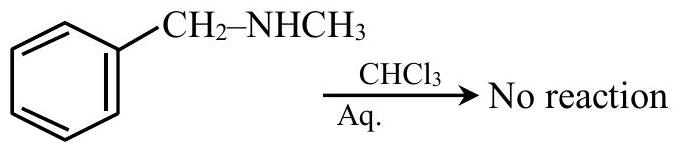
\includegraphics[max width=\textwidth, center]{2025_10_03_730bb016301631b89e24g-3(9)}\\
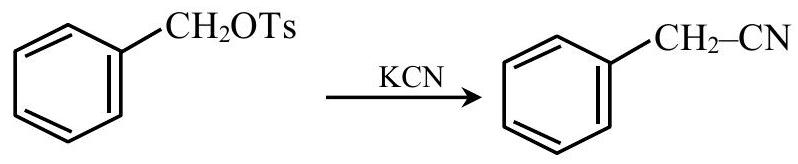
\includegraphics[max width=\textwidth, center]{2025_10_03_730bb016301631b89e24g-3(7)}\\
38. Given below are two statements : one is labelled as

Assertion (A) and the other is labelled as Reason (R).\\
Assertion (A) : In expensive scientific instruments, silica gel is kept in watch-glasses or in semipermeable membrane bags.

Reason (R) : Silica gel adsorbs moisture from air via adsorption, thus protects the instrument from water corrosion (rusting) and / or prevents malfunctioning. In the light of the above statements, choose the correct answer from the options given below :\\
(1) (A) is false but (R) is true\\
(2) (A) is true but (R) is false\\
(3) Both (A) and (R) are true and (R) is the correct explanation of (A)\\
(4) Both (A) and (R) are true but (R) is not the correct explanation of (A)

Official Ans. by NTA (3)\\
Allen Ans. (3)\\
Sol. Silica gel prevents water corrosion (rusting) and instrument malfunction by adsorbing moisture from the air.\\

\includegraphics{smile-2be77f2c50ba06ca808952704d60e13f19380215}

Caprolactam

\begin{figure}[h]
\begin{center}
  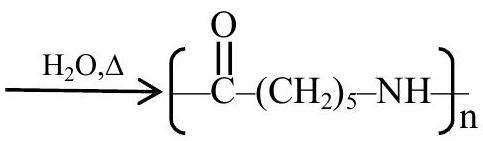
\includegraphics[width=\textwidth]{2025_10_03_730bb016301631b89e24g-3(8)}
\captionsetup{labelformat=empty}
\caption{Nylon -6}
\end{center}
\end{figure}

\begin{enumerate}
  \setcounter{enumi}{38}
  \item Match List I with List II
\end{enumerate}

\begin{center}
\begin{tabular}{|l|l|l|l|}
\hline
\multicolumn{2}{|c|}{List I} & \multicolumn{2}{|c|}{List II} \\
\hline
A & 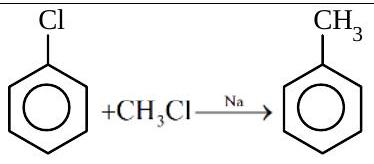
\includegraphics[max width=\textwidth]{2025_10_03_730bb016301631b89e24g-3(1)}
 & I & Fitting reaction \\
\hline
B & 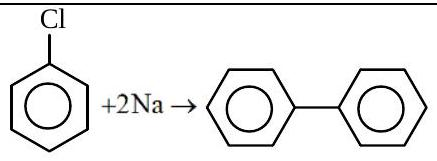
\includegraphics[max width=\textwidth]{2025_10_03_730bb016301631b89e24g-3(6)}
 & II & Wurtz Fitting reaction \\
\hline
C & 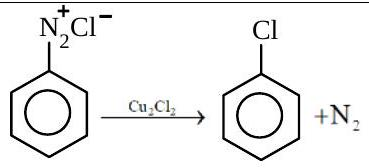
\includegraphics[max width=\textwidth]{2025_10_03_730bb016301631b89e24g-3}
 & III & Finkelstein reaction \\
\hline
D & \(\mathrm{C}_{2} \mathrm{H}_{5} \mathrm{Cl}+\mathrm{NaI} \rightarrow \mathrm{C}_{2} \mathrm{H}_{5} \mathrm{I}+\) NaCl & IV & Sandmeyer reaction \\
\hline
\end{tabular}
\end{center}

(1) A - II, B - I, C - III, D - IV\\
(2) A - III, B - II, C - IV, D - I\\
(3) A - IV, B - II, C - III, D - I\\
(4) \(\mathrm{A}-\mathrm{II}, \mathrm{B}-\mathrm{I}, \mathrm{C}-\mathrm{IV}, \mathrm{D}-\mathrm{III}\)

Official Ans. by NTA (4)\\
Allen Ans. (4)\\
Sol.

\begin{center}
\begin{tabular}{|l|l|l|}
\hline
\multicolumn{2}{|c|}{LIST-I} & LIST-II \\
\hline
A. & 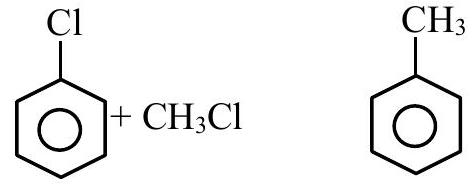
\includegraphics[max width=\textwidth]{2025_10_03_730bb016301631b89e24g-3(5)}
 & Wurtzfitting reaction \\
\hline
B. & 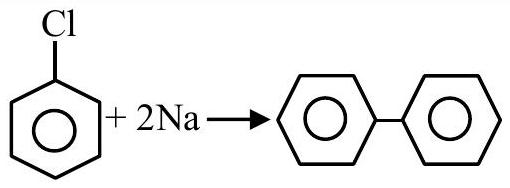
\includegraphics[max width=\textwidth]{2025_10_03_730bb016301631b89e24g-3(2)}
 & Fitting reaction \\
\hline
C. & 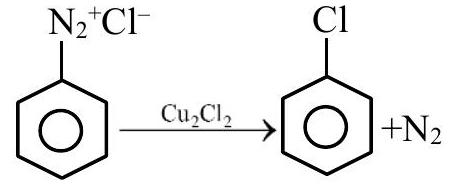
\includegraphics[max width=\textwidth]{2025_10_03_730bb016301631b89e24g-3(10)}
 & Sandmeyer reaction \\
\hline
D. & \(\mathrm{C}_{2} \mathrm{H}_{5} \mathrm{Cl}+\mathrm{NaI} \rightarrow \mathrm{C}_{2} \mathrm{H}_{5} \mathrm{I}+\mathrm{NaCl}\) & Finkelstein reaction \\
\hline
\end{tabular}
\end{center}

\begin{enumerate}
  \setcounter{enumi}{39}
  \item Caprolactam when heated at high temperature in presence of water, gives\\
(1) Teflon\\
(2) Dacron\\
(3) Nylon 6,6\\
(4) Nylon 6
\end{enumerate}

Official Ans. by NTA (4)\\
Allen Ans. (4)

Sol.\\
41. The alkaline earth metal sulphate(s) which are readily soluble in water is/are:\\
(A) \(\mathrm{BeSO}_{4}\)\\
(B) \(\mathrm{MgSO}_{4}\)\\
(C) \(\mathrm{CaSO}_{4}\)\\
(D) \(\mathrm{SrSO}_{4}\)\\
(E) \(\mathrm{BaSO}_{4}\)

Choose the correct answer from the options given below:\\
(1) A only\\
(2) B only\\
(3) A and B\\
(4) B and C

Official Ans. by NTA (3)\\
Allen Ans. (3)\\
Sol. Due to high hydration energy \(\mathrm{Be}^{2+}\) and \(\mathrm{Mg}^{2+}\), \(\mathrm{BeSO}_{4}\) and \(\mathrm{MgSO}_{4}\) are readily soluble in water.\\
42. Which of the following is correct order of ligand field strength?\\
(1) \(\mathrm{CO}<\) en \(<\mathrm{NH}_{3}<\mathrm{C}_{2} \mathrm{O}_{4}^{2-}<\mathrm{S}^{2-}\)\\
(2) \(\mathrm{S}^{2-}<\mathrm{C}_{2} \mathrm{O}_{4}^{2-}<\mathrm{NH}_{3}<\) en \(<\mathrm{CO}\)\\
(3) \(\mathrm{NH}_{3}<\) en \(<\mathrm{CO}<\mathrm{S}^{2-}<\mathrm{C}_{2} \mathrm{O}_{4}^{2-}\)\\
(4) \(\mathrm{S}^{2-}<\mathrm{NH}_{3}<\) en \(<\mathrm{CO}<\mathrm{C}_{2} \mathrm{O}_{4}^{2-}\)

Official Ans. by NTA (2)\\
Allen Ans. (2)\\
Sol. The increasing order of field strength of ligands (according to spectrochemical series)\\
\(\mathrm{S}^{2-}<\mathrm{C}_{2} \mathrm{O}_{4}^{2-}<\mathrm{NH}_{3}<\) en \(<\mathrm{CO}\)\\
43. Formation of photochemical smog involves the following reaction in which \(\mathrm{A}, \mathrm{B}\) and C are respectively.\\
(i) \(\mathrm{NO}_{2} \xrightarrow{\mathrm{hu}} \mathrm{A}+\mathrm{B}\)\\
(ii) \(\mathrm{B}+\mathrm{O}_{2} \rightarrow \mathrm{C}\)\\
(iii) \(\mathrm{A}+\mathrm{C} \rightarrow \mathrm{NO}_{2}+\mathrm{O}_{2}\)

Choose the correct answer from the options given below:\\
(1) \(\mathrm{O}, \mathrm{NO} \& \mathrm{NO}_{3}^{-}\)\\
(2) \(\mathrm{O}, \mathrm{N}_{2} \mathrm{O} \& \mathrm{NO}\)\\
(3) \(\mathrm{N}, \mathrm{O}_{2} \& \mathrm{O}_{3}\)\\
(4) \(\mathrm{NO}, \mathrm{O} \& \mathrm{O}_{3}\)

Official Ans. by NTA (4)\\
Allen Ans. (4)\\
Sol. \(\quad \mathrm{NO}_{2 \mathrm{~g}} \xrightarrow{\mathrm{hv}} \underset{(\mathrm{A})}{\mathrm{NO}_{\mathrm{g}}}+\underset{(\mathrm{B})}{\mathrm{O}_{\mathrm{g}}}\)\\
\(\underset{(\mathrm{B})}{\mathrm{O}_{\mathrm{g}}}+\mathrm{O}_{2 \mathrm{~g}} \rightleftharpoons \underset{(\mathrm{C})}{\mathrm{O}_{3 \mathrm{~g}}}\)

\[
\underset{(\mathrm{A})}{\mathrm{NO}_{\mathrm{g}}}+\underset{(\mathrm{C})}{\mathrm{O}_{3 \mathrm{~g}}} \longrightarrow \mathrm{NO}_{2 \mathrm{~g}}+\mathrm{O}_{2 \mathrm{~g}}
\]

\begin{enumerate}
  \setcounter{enumi}{43}
  \item During the qualitative analysis of \(\mathrm{SO}_{3}^{2-}\) using dilute \(\mathrm{H}_{2} \mathrm{SO}_{4}, \mathrm{SO}_{2}\) gas is evolved which turns \(\mathrm{K}_{2} \mathrm{Cr}_{2} \mathrm{O}_{7}\) solution (acidified with dilute \(\mathrm{H}_{2} \mathrm{SO}_{4}\) ):\\
(1) Black\\
(2) Red\\
(3) Green\\
(4) Blue
\end{enumerate}

Official Ans. by NTA (3)\\
Allen Ans. (3)\\
Sol. \(\mathrm{Cr}_{2} \mathrm{O}_{7}^{2-}+\mathrm{SO}_{3}^{2-} \xrightarrow{\mathrm{H}^{+}} \underset{\text { Green }}{\mathrm{Cr}^{3+}}+\mathrm{SO}_{4}^{2-}\)\\
45. To inhibit the growth of tumours, identify the compounds used from the following:\\
(A) EDTA\\
(B) Coordination Compounds of Pt\\
(C) D-Penicillamine\\
(D) Cis - Platin

Choose the correct answer from the option given below:\\
(1) B and D Only\\
(2) C and D Only\\
(3) A and B Only\\
(4) A and C Only

Official Ans. by NTA (1)\\
Allen Ans. (1)\\
Sol. Cis - Platin is used in chemotherapy to inhibits the growth of tumors. \(\left(\operatorname{cis}\left[\operatorname{Pt}\left(\mathrm{NH}_{3}\right)_{2} \mathrm{Cl}_{2}\right]\right)\)\\
46. In the wet tests for identification of various cations by precipitation, which transition element cation doesn't belong to group IV in qualitative inorganic analysis?\\
(1) \(\mathrm{Fe}^{3+}\)\\
(2) \(\mathrm{Zn}^{2+}\)\\
(3) \(\mathrm{Co}^{2+}\)\\
(4) \(\mathrm{Ni}^{2+}\)

Official Ans. by NTA (1)\\
Allen Ans. (1)\\
Sol. \(\mathrm{Zn}^{2+}, \mathrm{Co}^{2+}, \mathrm{Ni}^{2+}=\mathrm{IV}^{\text {th }}\) Group\\
\(\mathrm{Fe}^{3+}=\mathrm{III}{ }^{\mathrm{rd}}\) Group\\
47. Match List I with List II

\begin{center}
\begin{tabular}{|l|l|l|l||}
\hline
\multicolumn{2}{|c|}{\begin{tabular}{c}
LIST-I \\
(molecules/ions) \\
\end{tabular}} & \multicolumn{2}{c|}{\begin{tabular}{c}
LIST-II \\
(No. of lone pairs of e \\
on central atom) \\
\end{tabular}} \\
\hline
(A) & \(\mathrm{IF}_{7}\) & I. & Three \\
\hline
(B) & \(\mathrm{ICl}_{4}^{-}\) & II. & One \\
\hline
(C) & \(\mathrm{XeF}_{6}\) & III. & Two \\
\hline
(D) & \(\mathrm{XeF}_{2}\) & IV. & Zero \\
\hline
\end{tabular}
\end{center}

Choose the correct answer from the options given below:\\
(1) \(\mathrm{A}-\mathrm{II}, \mathrm{B}-\mathrm{III}, \mathrm{C}-\mathrm{IV}, \mathrm{D}-\mathrm{I}\)\\
(2) \(\mathrm{A}-\mathrm{IV}, \mathrm{B}-\mathrm{III}, \mathrm{C}-\mathrm{II}, \mathrm{D}-\mathrm{I}\)\\
(3) A - II, B - I, C - IV, D - III\\
(4) \(\mathrm{A}-\mathrm{IV}, \mathrm{B}-\mathrm{I}, \mathrm{C}-\mathrm{II}, \mathrm{D}-\mathrm{III}\)

Official Ans. by NTA (2)\\
Allen Ans. (2)\\
Sol. \(\mathrm{IF}_{7}\) zero lone pair\\
\(\mathrm{ICl}_{4}^{-} \quad\) two lone pair\\
\(\mathrm{XeF}_{6} \quad\) one lone pair\\
\(\mathrm{XeF}_{2}\) three lone pair\\
48. For \(\mathrm{OF}_{2}\) molecule consider the following:\\
(A) Number of lone pairs on oxygen is 2 .\\
(B) FOF angle is less than \(104.5^{\circ}\).\\
(C) Oxidation state of O is -2 .\\
(D) Molecule is bent ' \(V\) ' shaped.\\
(E) Molecular geometry is linear.

Correct options are:\\
(1) C, D, E only\\
(2) B, E, A only\\
(3) A, C, D only\\
(4) A, B, D only

Official Ans. by NTA (4)\\
Allen Ans. (4)

Sol.\\

\includegraphics{smile-1464414e6640476239ac7260dd5b3f69e0cea557}

\begin{itemize}
  \item Two lone pair one oxygen
  \item Molecule is ' v ' shaped
  \item Bond angle is less than \(104.5^{\circ}\left(102^{\circ}\right)\)
  \item \(\mathrm{O} \cdot \mathrm{S} \cdot\) of ' O ' is +2
\end{itemize}

\begin{enumerate}
  \setcounter{enumi}{48}
  \item Lithium aluminium hydride can be prepared from the reaction of\\
(1) LiCl and \(\mathrm{Al}_{2} \mathrm{H}_{6}\)\\
(2) LiH and \(\mathrm{Al}_{2} \mathrm{Cl}_{6}\)\\
(3) \(\mathrm{LiCl}, \mathrm{Al}\) and \(\mathrm{H}_{2}\)\\
(4) LiH and \(\mathrm{Al}(\mathrm{OH})_{3}\)
\end{enumerate}

Official Ans. by NTA (2)\\
Allen Ans. (2)\\
Sol. \(8 \mathrm{LiH}+\mathrm{Al}_{2} \mathrm{Cl}_{6} \longrightarrow 2 \mathrm{LiAlH}_{4}+6 \mathrm{LiCl}\)\\
50. Match List - I with List - II

\begin{center}
\begin{tabular}{|l|l|l|l|}
\hline
\multicolumn{2}{|r|}{LIST-I (Atomic number)} & \multicolumn{2}{|r|}{LIST-II (Block of periodic table)} \\
\hline
(A) & 37 & I. & p-block \\
\hline
(B) & 78 & II. & d-block \\
\hline
(C) & 52 & III. & f-block \\
\hline
(D) & 65 & IV. & s-block \\
\hline
\end{tabular}
\end{center}

Choose the correct answer from the options given below:\\
(1) \(\mathrm{A}-\mathrm{II}, \mathrm{B}-\mathrm{IV}, \mathrm{C}-\mathrm{I}, \mathrm{D}-\mathrm{III}\)\\
(2) \(\mathrm{A}-\mathrm{I}, \mathrm{B}-\mathrm{III}, \mathrm{C}-\mathrm{IV}, \mathrm{D}-\mathrm{II}\)\\
(3) \(\mathrm{A}-\mathrm{IV}, \mathrm{B}-\mathrm{III}, \mathrm{C}-\mathrm{II}, \mathrm{D}-\mathrm{I}\)\\
(4) \(\mathrm{A}-\mathrm{IV}, \mathrm{B}-\mathrm{II}, \mathrm{C}-\mathrm{I}, \mathrm{D}-\mathrm{III}\)

Official Ans. by NTA (4)\\
Allen Ans. (4)\\
Sol.

\begin{center}
\begin{tabular}{|c|c|}
\hline
Atomic number & Block \\
\hline
\(37(\mathrm{~K})\) & s-block \\
\hline
\(78(\mathrm{Pt})\) & d-block \\
\hline
\(52(\mathrm{Te})\) & p-block \\
\hline
\(65(\mathrm{~Tb})\) & f-block \\
\hline
\end{tabular}
\end{center}

\section*{SECTION-B}
\begin{enumerate}
  \setcounter{enumi}{50}
  \item Consider the cell\\
\(\mathrm{Pt}_{(\mathrm{s})}\left|\mathrm{H}_{2}(\mathrm{~g}, 1 \mathrm{~atm})\right| \mathrm{H}^{+}(\mathrm{aq}, 1 \mathrm{M})| | \mathrm{Fe}^{3+}(\mathrm{aq}), \mathrm{Fe}^{2+}(\mathrm{aq}) \mid \mathrm{Pt}(\mathrm{s})\)\\
When the potential of the cell is 0.712 V at 298 K , the ratio \(\left[\mathrm{Fe}^{2+}\right] /\left[\mathrm{Fe}^{3+}\right]\) is \(\_\_\_\_\) .\\
(Nearest integer)\\
Given: \(\mathrm{Fe}^{3+}+\mathrm{e}^{-}=\mathrm{Fe}^{2+}, \mathrm{E}^{\circ} \mathrm{Fe}^{3+}, \mathrm{Fe}^{2+} \mid \mathrm{Pt}=0.771\)\\
\(\frac{2.303 R T}{F}=0.06 \mathrm{~V}\)\\
Official Ans. by NTA (10)\\
Allen Ans. (10)\\
Sol\\
\(\mathrm{Pt}_{(\mathrm{s})}\left|\mathrm{H}_{2}(\mathrm{~g}, 1 \mathrm{~atm})\right| \mathrm{H}^{+}(\mathrm{aq}, 1 \mathrm{M}) \| \mathrm{Fe}^{3+}(\mathrm{aq}), \mathrm{Fe}^{2+}(\mathrm{aq}) \mid \mathrm{Pt}\)\\
at anode \(\mathrm{H}_{2} \longrightarrow 2 \mathrm{H}^{+}+2 \mathrm{e}^{-}\)\\
At cathode \(\mathrm{Fe}_{\mathrm{aq}}^{3+}+\mathrm{e}^{-} \longrightarrow \mathrm{Fe}_{\mathrm{aq}}^{2+}\)\\
\(\mathrm{E}^{\circ}=\mathrm{E}_{\mathrm{H}_{2} \mid \mathrm{H}^{+}}^{\circ}+\mathrm{E}_{\mathrm{Fe}^{3+} \mid \mathrm{Fe}^{2+}}^{\circ}=0 \cdot 771 \mathrm{~V}\)\\
\(\mathrm{E}=\mathrm{E}^{\circ}-\frac{0.06}{1} \log \frac{\mathrm{Fe}^{2+}}{\mathrm{Fe}^{3+}}\)\\
\(0 \cdot 712=(0+0 \cdot 771)-\frac{0 \cdot 06}{1} \log \frac{\mathrm{Fe}^{2+}}{\mathrm{Fe}^{3+}}\)\\
\(\log \frac{\mathrm{Fe}^{2+}}{\mathrm{Fe}^{3+}}=\frac{0 \cdot 059}{0 \cdot 06} \approx 1\)\\
\(\frac{\mathrm{Fe}^{2+}}{\mathrm{Fe}^{3+}}=10\)
  \item A 300 mL bottle of soft drink has \(0.2 \mathrm{M} \mathrm{CO}_{2}\) dissolved in it. Assuming \(\mathrm{CO}_{2}\) behaves as an ideal gas, the volume of the dissolved \(\mathrm{CO}_{2}\) at STP is\\
\(\_\_\_\_\) mL. (Nearest integer)
\end{enumerate}

Given: At STP, molar volume of an ideal gas is \(22.7 \mathrm{~L} \mathrm{~mol}^{-1}\)

Official Ans. by NTA (1362)\\
Allen Ans. ( 1362 ml )\\
Sol. Mole of \(\mathrm{CO}_{2}=0.2 \mathrm{M} \times\left(300 \times 10^{-3}\right) \mathrm{L}\)\\
= 0.06 Mole

Volume of 0.06 mole \(\mathrm{CO}_{2}\) at S.T.P

\[
\begin{aligned}
& =0.06 \times 22.7 \\
& =1.362 \mathrm{~L}
\end{aligned}
\]

\begin{enumerate}
  \setcounter{enumi}{52}
  \item A solution containing 2 g of a non-volatile solute in 20 g of water boils at 373.52 K . The molecular mass of the solute is \(\_\_\_\_\) \(\mathrm{g} \mathrm{mol}^{-1}\). (Nearest integer)
\end{enumerate}

Given, water boils at \(373 \mathrm{~K}, \mathrm{~K}_{\mathrm{b}}\) for water \(=0.52 \mathrm{~K} \mathrm{~kg} \mathrm{~mol}^{-1}\)

Official Ans. by NTA ( \(\mathbf{1 0 0 g}\) )\\
Allen Ans. ( \(\mathbf{1 0 0 g}\) )\\
Sol. \(\Delta \mathrm{T}_{\mathrm{b}}=373.52-373\)

\[
=0.52
\]

\(\Delta \mathrm{T}_{\mathrm{b}}=\mathrm{Kb} \cdot \mathrm{m}\)\\
\(0.52=0.52 \times \frac{2}{\text { Molar Mass }} \times \frac{1}{20 \times 10^{-3}}\)\\
Molar Mass \(=100 \mathrm{~g} / \mathrm{mol}\)\\
54. If compound A reacts with B following first order kinetics with rate constant \(2.011 \times 10^{-3} \mathrm{~s}^{-1}\). The time taken by A (in seconds) to reduce from 7 g to 2 g will be \(\_\_\_\_\) (Nearest Integer)\\
\([\log 5=0.698, \log 7=0.845, \log 2=0.301]\)\\
Official Ans. by NTA (623)\\
Allen Ans. (623)\\
Sol.

\[
A+B \rightarrow P
\]

\(\mathrm{t}=0\)\\
7g\\
\(\mathrm{t}=\mathrm{t}\)\\
2 g\\
at constant volume

\[
\begin{aligned}
\mathrm{t} & =\frac{2.303}{\mathrm{~K}} \log \frac{[\mathrm{~A}]_{0}}{[\mathrm{~A}]_{\mathrm{t}}} \\
& =\frac{2 \cdot 303}{2 \cdot 011 \times 10^{-3}} \log \frac{7}{2} \\
& =\frac{2 \cdot 303 \times 0 \cdot 544}{2 \cdot 011 \times 10^{-3}} \\
& =622.989 \\
& \approx 623
\end{aligned}
\]

\begin{enumerate}
  \setcounter{enumi}{54}
  \item The energy of one mole of photons of radiation of frequency \(2 \times 10^{12} \mathrm{~Hz}\) in \(\mathrm{J} \mathrm{mol}^{-1}\) is \(\_\_\_\_\) .\\
(Nearest integer)\\
(Given: \(\mathrm{h}=6.626 \times 10^{-34} \mathrm{Js}\)\\
\(\mathrm{N}_{\mathrm{A}}=6.022 \times 10^{23} \mathrm{~mol}^{-1}\) )\\
Official Ans. by NTA (798)\\
Allen Ans. (798)\\
Sol. For one photon \(\mathrm{E}=\mathrm{hv}\)\\
For one mole photon,
\end{enumerate}

\[
\begin{aligned}
\mathrm{E} & =6 \cdot 023 \times 10^{23} \times 6 \cdot 626 \times 10^{-34} \times 2 \times 10^{12} \\
& =798 \cdot 16 \mathrm{~J} \\
& \approx 798 \mathrm{~J}
\end{aligned}
\]

\begin{enumerate}
  \setcounter{enumi}{55}
  \item The number of electrons involved in the reduction of permanganate to manganese dioxide in acidic medium is \(\_\_\_\_\) .\\
Official Ans. by NTA (3)\\
Allen Ans. (3)\\
Sol. \(\stackrel{+7}{\mathrm{MnO}} \mathrm{O}_{4}^{-}+4 \mathrm{H}^{+}+3 \mathrm{e}^{-} \longrightarrow \stackrel{+4}{\mathrm{MnO}} \mathrm{O}_{2}+2 \mathrm{H}_{2} \mathrm{O}\)
  \item When 2 litre of ideal gas expands isothermally into vacuum to a total volume of 6 litre, the change in internal energy is \(\_\_\_\_\) J. (Nearest integer)
\end{enumerate}

Official Ans. by NTA (0)\\
Allen Ans. (0)\\
Sol. For ideal gas \(\mathrm{U}=\mathrm{f}(\mathrm{T})\)\\
and for isothermal process, \(\Delta \mathrm{U}=0\)\\
58. 600 mL of 0.01 M HCl is mixed with 400 mL of \(0.01 \mathrm{M} \mathrm{H}_{2} \mathrm{SO}_{4}\). The pH of the mixture is\\
\(\_\_\_\_\) \(\times 10^{-2}\). (Nearest integer)\\[0pt]
[Given \(\log 2=0.30, \quad \log 3=0.48\)\\
\(\log 5=0.69 \quad \log 7=0.84\)\\
\(\log 11=1.04]\)\\
Official Ans. by NTA (186)\\
Allen Ans. (186)\\
Sol. Total milimoles of \(\mathrm{H}^{+}=(600 \times 0.01)+(400 \times 0.01 \times 2)\)

\[
\begin{aligned}
& =14 \\
& {\left[\mathrm{H}^{+}\right]=\frac{14}{1000}=14 \times 10^{-3}} \\
& \mathrm{pH}=3-\log 14 \\
& =1.86 \\
& =186 \times 10^{-2}
\end{aligned}
\]

\begin{enumerate}
  \setcounter{enumi}{58}
  \item A trisubstituted compound 'A', \(\mathrm{C}_{10} \mathrm{H}_{12} \mathrm{O}_{2}\) gives neutral \(\mathrm{FeCl}_{3}\) test positive. Treatment of compound 'A' with NaOH and \(\mathrm{CH}_{3} \mathrm{Br}\) gives \(\mathrm{C}_{11} \mathrm{H}_{14} \mathrm{O}_{2}\), with hydroiodic acid gives methyl iodide and with hot conc. NaOH gives a compound \(\mathrm{B}, \mathrm{C}_{10} \mathrm{H}_{12} \mathrm{O}_{2}\). Compound 'A' also decolorises alkaline \(\mathrm{KMnO}_{4}\). The number of \(\pi\) bond/s present in the compound ' A ' is \(\_\_\_\_\) .
\end{enumerate}

59 Official Ans. by NTA (4)\\
Allen Ans. (4)\\
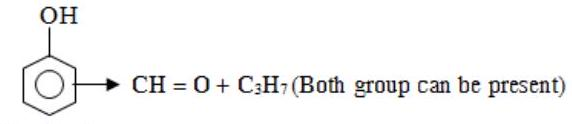
\includegraphics[max width=\textwidth, center]{2025_10_03_730bb016301631b89e24g-7(1)}\\
( \(\mathrm{C}_{10} \mathrm{H}_{12} \mathrm{O}_{2}\) )\\
(or)\\

\includegraphics{smile-5d304e640e28bfb4f26d9a33e6460718b2130853}\\
\(\mathrm{CH}_{2} \mathrm{OH}+\mathrm{C}=\mathrm{C}-\mathrm{CH}_{3}\) (Both group can be present)

\begin{figure}[h]
\begin{center}
\captionsetup{labelformat=empty}
\caption{( (\textbackslash mathrm\{C}\textit{\{10\} \textbackslash mathrm\{H\}}\{12\} \textbackslash mathrm\{O\}\_\{2\}) )\}\\
  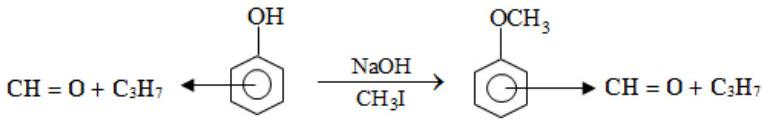
\includegraphics[width=\textwidth]{2025_10_03_730bb016301631b89e24g-7}
\end{center}
\end{figure}

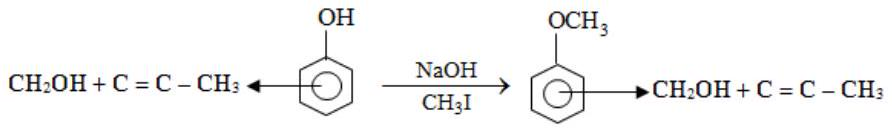
\includegraphics[max width=\textwidth, center]{2025_10_03_730bb016301631b89e24g-7(2)}\\
60. Some amount of dichloromethane \(\left(\mathrm{CH}_{2} \mathrm{Cl}_{2}\right)\) is added to 671.141 mL of chloroform \(\left(\mathrm{CHCl}_{3}\right)\) to prepare \(2.6 \times 10^{-3} \mathrm{M}\) solution of \(\mathrm{CH}_{2} \mathrm{Cl}_{2}(\mathrm{DCM})\). The concentration of DCM is \(\_\_\_\_\) ppm (by mass).

Given: Atomic mass : \(\mathrm{C}=12 ; \mathrm{H}: 1 ; \mathrm{Cl}=35.5\) density of \(\mathrm{CHCl}_{3}=1.49 \mathrm{~g} \mathrm{~cm}^{-3}\)

Official Ans. by NTA (221)\\
Allen Ans. (148)\\
Sol. \(\quad\) Molarity \(=\frac{\text { mole }}{\text { volume }}\)

\[
\begin{aligned}
2.6 \times 10^{-3} & =\frac{\mathrm{x} / 85}{0.67141} \\
\mathrm{x} & =0.148 \mathrm{~g}
\end{aligned}
\]

conc. Fo DCM in ppm \(=\frac{0.148}{1.49 \times 671.141} \times 10^{6}\)\\
\(=148 \mathrm{ppm}\)


\end{document}